\chapter{Conclusion and future work}\label{ch:conclusion}

\begin{figure}[h!]
\centering
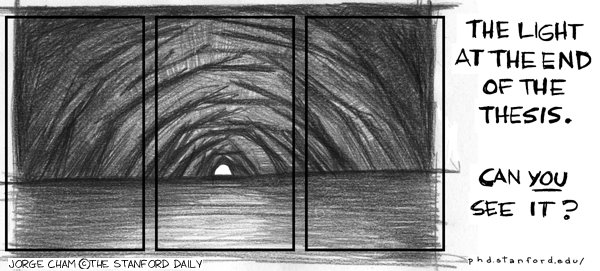
\includegraphics[width=.8\textwidth]{./gfx/Chapter07/phd051700s.jpg}
\caption{A  comic strip by Jorge Cham from his series ``Piled Higher and Deeper'' \cite{Cham}}
\end{figure}

The main goal of this thesis was to explore appearance-based methods in the novel contexts of wearable and hand-held object recognition and visual localization, with emphasis on whether biologically-inspired algorithms can have a positive impact on performance. Therefore, around this idea we defined individual hypotheses for the work described in each chapter. As means to achieve this objective we collected two large datasets; provided a thorough evaluation of baseline and custom-created image description methods; developed a biologically inspired model of place cells for visual localization and produced a prototype system for assistive localization using wearable/hand-held visual input and tactile feedback.

In this final section we will extend this summary for each of these contributions and address some future perspectives.

\section{Summary of contributions}

\begin{enumerate}
\item \textbf{Context based image retrieval (CBIR) methods for wearable and assistive applications} First, we have analysed the impact of computer vision in mobile and wearable technologies in an assistive context, providing complete studies of appearance-based methods for two key applications, hand-held object recognition of household products and indoor navigation.

\item \textbf{Artificial Place Cell Model} Second, we have provided a novel artificial place cell (APC) model for their biological counterparts found in the hippoccampus, and tested it under the same challenging conditions of indoor navigation by using a generalised regression neural network as a training mechanisms for learning a positional ground truth from a database.

\item \textbf{Prototype of an assistive application} Third, we took this previous findings to the next step and develop a prototype client-server Android application for assistive localization from wearable and hand-held devices using their visual input and a haptic feedback tablet to provide tactile cues to the location estimates. With this work we laid out the foundations for an achievable solution from the commercial perspective and stressed the importance of inclusive design.


\item \textbf{Two novel datasets} These contributions are accompanied by two important datasets, namely the SHORT dataset for hand-held object recognition and the RSM dataset of \emph{visual paths}.
\end{enumerate}

As we can see, from the computer vision application development pipeline devised in Figure ~\ref{fig:cv_dev_pipeline} we have accomplished all the stages.

\section{Concluding remarks}

\subsection{Context based image retrieval (CBIR) methods for wearable and assistive applications}

The research question for Chapters \ref{ch:chapter2},~\ref{ch:chapterSHORT},~\ref{ch:chapter4} was whether the appearance-based CBIR methods extensively used in the object recognition field could be applied to the challenging scenarios of wearable and assistive applications, with emphasis in two key applications: object recognition and visual indoor localisation. Therefore in Chapter \ref{ch:chapter2} we studied the particularities of this use case, and defined simple image matching methods and metrics and test them with prototype data so we could specify the data and performance requirements for the more thorough evaluation carried out in the following chapters.

The work described in Chapter~\ref{ch:chapter3} focuses on hand-held object recognition. We described the acquisition of the SHORT dataset and the evaluation of popular appearance-based methods against this dataset. The dataset proved to be extremely challenging even for algorithms that had practically solved other datasets. With the arrival of new datasets such as SHORT and ImageNet, these algorithms's performance decay, and the community had to put focus on more flexible learning methods particularly deep learning.

In Chapter~\ref{ch:chapter4} we studied another important application, indoor visual localization from hand-held and wearable cameras. We acquired another large dataset, the RSM dataset, built a benchmark and developed a series of appearance-based methods and metrics we believe are more descriptive than the current state of the art. In the benchmark, we showed how our custom methods outperformed standard methods such as dense SIFT or HOG3D, but also the state of the art SLAM method for indoor scnearios, LSD-SLAM (the top performing one, SF-GABOR, exhibited a localisation error $\mu_{e,SF-GABOR} = 1.31 $ m whilst LSD-SLAM $< \mu_{e,LSD-SLAM} = 2.48 $ m).  We also argued that the power of SLAM resides in the robustness of its tracking mechanisms. Our methods, on the other hands have shown good results when tested in isolation, where no tracking was applied; therefore we believe they can work alongside SLAM to reduce estimation errors during SLAM's optimisation stages, the same way OpenFABMAP is used in the own LSD-SLAM.


\subsection{Artificial Place Cell Model}

In Chapter~\ref{ch:chapter5} we enunciated a different research hypothesis, which is in reality twofold. In first place, we questioned ourselves whether it was possible to find  a model of biological place cells using the appearance-based methods described in Chapter~\ref{ch:chapter4}. In particular, we were interested in analysing the behaviour of the kernel similarity metric when frame encoding vectors, or histograms of visual words, were used as inputs. The second research question was whether this artificial place cell models could provide localisation by mimicking the behaviour found in biology.

As we showed, the answer to the two questions was positive. We effectively constructed what we call artificial place cells (APCs), physical models of their biological counterparts, the biological place cells (BPCs). We tested them with our RSM dataset and showed how they could provide localisation by associating views from a crowdsourced database. In particular, the models mimick the BPCs firing rate, showing a tuning curve-type function that peaks on locations that are closer to that of the query we are trying to estimate. Once the APCs were characterised, we presented two localisation models. One is based on the maximum response of the APB tuning curve, and the other is based on a generalistic regression neural network (GRNN) that has the advantage of providing sublocalisation -- i.e. training the neural network regressor with a discrete number of APCs we are able to provide continuous localisation for a given query. We also provide a complete evaluation using the descriptors described in Chapter~\ref{ch:chapter4} and establish a comparison with LSD-SLAM.

We believe the findings described in Chapter~\ref{ch:chapter5} represent the first model of APCs that relies purely on vision to provide localisation estimates. However, many questions remain unanswered, opening many lines for future work that we will describe in the next section. 

\subsection{Prototype of an assistive application}

In Chapter~\ref{ch:chapter6} we described how taking the localisation pipeline presented in Chapter \ref{ch:chapter4} we developed an assistive localisation prototype that used vision as input and haptic feedback to provide the user with a location estaimte. With a client-server architecture, the visual input can be provided from a wearable camera or mobile or tablet camera, processed in the server which sends the location estimation to the Senseg, a tactile feedback Android tablet that is able to provide a range of different textures that the user can learn to interpret depending of the application.

We provided a description of the prototype and their results in a ``live'' scenario, and also an experiment on tactile feedback perception. The purpose of this experiment was to assess whether it is possible to use a device such as the Senseg to provide location estimations along one dimension, i.e. how far along the path the subject is. 

The results showed that up to a certain extent (a precision of roughly 3 m) the users were able to distinguish neighbouring posisitions on the tactile tablet. However, we believe this only represents a pilot study and many questions should be addressed before this is tested with blind and partially sighted users. We will describe future work in the next section.

\subsection{Datasets}

\subsubsection{SHORT dataset}

In the case of SHORT, we took a slightly different approach and diverged from the trend in object recognition dataset research. Instead of going towards the domain and dataset depth of big data (although our datasets are not small, containing hundreds of thousands of examples), we emphasise the need of understanding better the constraints of the problem at hand (wearable or hand-held object recognition) and also comprehend why even state-of-the art deep learning approaches that purely learn from examples find it hard to generalise outside the dataset they're being trained --and tested- on. Torralba and Efros already studied the perils of dataset bias and poor cross-dataset generalisation \cite{torralba2011unbiased} and these were one of the main motivations to build the SHORT dataset as there were no available dataset that could capture the challenges of wearable or hand-held recognition of groceries.

With the expansion of SHORT from 30 to 100 categories the category depth problem was solved, allowing for enough generalisation challenge from within the dataset. The test set, with more than	 130,000 images constitutes an extremely challenging results, with some preliminary work  being carried out in our group demonstrating the poor performance of deep learning frameworks such as Berkeley's Caffe \cite{jia2014caffe}.

\section{Future work}

Finally, we will summarise here the future work for each line of work previously described in each corresponding chapter.

\subsection{Datasets}

One might think that a straightforward future work for a dataset is just carry out an expansion. We think that this is one of the key aspects for the growth and dissemination of the data. However, we need to take into account the current challenges and opportunities of crowdsourcing techniques and big data scenarios.

\subsubsection{SHORT dataset}

A large proportion of the time dedicated to the acquisition of SHORT was invested in prototypes of the acquisition set-up and trials for its testing. The intention was to have a flexible but at the same time reproducible set-up, as it can be shown in Fig. \ref{fig:acqsetup}. As the number of categories in the last version of SHORT, SHORT-100 was deemed appropriate in terms of generalisation under our testing conditions, we decided to stop its development there. However, the more categories we have in the training dataset the better for this type of benchmarks (controlled training set \textit{vs.} natural or \textit{wild} test set) to be adopted. Therefore it is important to contact large suppliers of product images to supermarket and retail chains and propose collaboration plans beneficial to both the research community (these suppliers are capable of taking our approach to scale) and for the image suppliers, as they can have an important role in acquiring the models for future improved training algorithms.

Regarding the test set, a natural expansion would consist of the setup of a web repository and the development of a retrieval mobile app so images of new grocery products could be contributed to the platform.

In this respect, there are open-source alternatives such as \cite{apple} and \cite{google} that would facilitate this task as instead of developing a dedicated app, the SHORT test set acquisition can be a project within these initiatives and attract altruist contributors that might have an interest on this sort of projects.

Alternatively, modern mobile app and web technologies allow for easy deployment of apps based on client-server communication using a RESTful architecture. By creating an API, posting images would be trivial, and the development of the client would be the final user's choice.

\subsubsection{RSM dataset}
\label{sec:futureRSM}
For the RSM dataset, we envisage that a larger number of corridors could attract more users. We are currently developing synthetic data of similar-looking corridors to assess the performance of appearance-based localisation, with and without employing artificial place cell models. The passes of this synthetic journey will be incorporated into the publicly available RSM dataset repository for the community to evaluate their algorithms in both real and synthetic datasets. These passes contain ground truth information and we are including different camera movements in some of the passes to mimic human head movements that have an effect on wearable camera footage.

Its expansion should idealy contain more variety of places, lighting conditions and overall, devices. In fact, this is an opportunity for crowdsourcing too, as a collection app or API as described in the previous section, could on its own encourage the contribution of many different devices in the process.

Also one of the biggest challenges and opportunities is to expand the dataset with 2 o 3D ground truth but maintaining the natural particularities of human motion. Rich 3D ground truth have traditionally been provided by robots, depriving these datasets from real human motion artifacts. We are currently exploring depth sensor and multi-camera indoor datasets in our research group for the purposes of indoor tracking of human subjects, and we believe this information could be incorporated to our dataset to provide a richer ground truth and motivate additional projects such as the creation of multi-modal signatures between external human tracking, visual input and sensor readings.

The acquisition of this sensor data could add huge value to the dataset. It is easy to collect sensor reading: APIs are mature in mobile phone development kits, and at the same time would attract research from the sensor, the ``Internet of Things'' (IoT) and big data communities.

One of our future ideas to develop within our research group, is the modelling of similar tuning curves as the ones produced by the place cells, but on sensor data. The relationship between both sources of curves could have a huge impact in learning locations without the need of a map or even a database not obtained through crowdsourcing.

\subsection{Appearance-based methods for visual localisation}
As we are open sourcing the evaluation pipeline, we welcome different research groups to contribute code to expand the amount of appearance-based methods for visual localisation.

A second future line of work will be to test our best performing method in conjunction with SLAM, the same way Open FAB-MAP is used with LSD-SLAM. We believe the SLAM community should keep relying on appearance-based methods not only for loop closure tasks but to povide their localisation and mapping with some semantic information about the environment.

A third project that would naturally emanate from this work would be a hierarchical appearance-based localisation that would implement the latest advances in scene retrieval and multi-sensor positioning. The same way we are providing a localisation within one journey from a database of similar journeys, we could also provide localisation within a building, within a city and so on. Broader estimates can come from GRNN signals, Wi-Fi and other radio location-based services, whilst fine grained positioning can be provided by appearance-based methods and a combination of these with SLAM when a database is not present.

\subsection{Biologically inspired localization methods based on place cell models}

We are currently studying different normalisation methods for the artificial place cell models and we recently submitted a paper with our latest advances in this area~\cite{Rivera-Rubio2015tnnls}. 
Fisher Vector as method (GMM more biologically plausible?). 

In another line of future work, we are exploring different normalisation and matrix equilibration techniques by which the localisation using APCs can be optimised. In particular, divisive normalisation has been proposed as a model to describe non-linear population coding effects observed within biological sensory neurons. Different forms of normalisation have also been applied in machine learning, such as $L_2$ normalisation across features for each sample. In this current project, we explore the relationship between divisive normalisation and matrix equilibration, a technique that scales matrix rows and columns. Using mixed matrix norms, and introducing partial mixed matrix norms, we interpret divisive normalisation in terms of matrix equilibration. We evaluate the effect of divisive normalisation in our artificial place cells models. We hypothesise that the use of partial mixed norms provide methods of scaling ensembles of neurons and their responses over experiments in a variety of ways, some of which may improve the performance of artificial networks. We believe that the freedom to select different combinations of norms provides the potential to improve performance, but improvements are both highly context dependent, and network dependent. This is the reason for testing these techniques on our recently acquired synthetic corridor to be incorporated into the RSM dataset which we described in previous Section \ref{sec:futureRSM}.


\subsection{Assitive localization apps with visual input and haptic feedback}

\td{}{ToDo}{Reword}
In future work, we plan to extend two aspects of the work reported in this thesis: improving the visual processing and further exploring the capabilities of mapping visual information onto haptic devices. Generally speaking, the use of images captured with wearable cameras by a navigating person remains only superficially explored in the literature. Though power consumption and accuracy of detection remain key barriers to wide scale deployment, these barriers will be lessened over time. In addition to location estimation, the possibility of detecting obstructions, people and any deviations in environment from previous journeys holds great promise. In future work, we plan to integrate ground-plane detection on a wearable camera in order to detect irregularities in walking surface, or obstructions out to around a 5 m distance. Furthermore, other sources of data, for example Wi-Fi signal strength, can play a key role in both improving the reliability of position estimation, and robustness in the case of indoor lighting failure.

On the haptic side, we plan to refine the mapping from floor plans to tactile feedback. Returning to the Senseg\texttrademark~ platform as an example, a variety of textures could be conveyed to a user by varying the amplitude and temporal pattern of voltage pulses sent to the haptic interface. By combining the flexibility of this device with prior work on mapping textures to haptic feedback, it should be possible to improve the information conveyed to a visually impaired user by automatically harvesting visual information from an appropriately prepared map. For example, a standard map format that contains hatches or textures to illustrate locations of steps, or different types of rooms could be mapped to different tactile sensations on the device. Combining this information with lists of possible journeys that might be taken allows journey planning to be performed, and more readily opens up exploration of indoor locations.


